\documentclass[11pt,a4paper,oneside]{article}
\usepackage[utf8]{inputenc}
\usepackage[T1]{fontenc}
\usepackage[french]{babel}
\usepackage{lmodern}
\usepackage{microtype}
\usepackage[a4paper,margin=2.25cm,headheight=15pt,footskip=28pt]{geometry}
\usepackage{amsmath,amssymb,amsthm,mathtools}
\usepackage{booktabs,tabularx,array}
\usepackage[dvipsnames]{xcolor}
\usepackage{tikz}
\usepackage{graphicx}
\usetikzlibrary{arrows.meta,calc,intersections,angles,quotes,patterns,positioning,decorations.pathreplacing}
\usepackage{fancyhdr}
\usepackage{hyperref}
\usepackage{enumitem}

\definecolor{Forest}{HTML}{1D5B4A}
\definecolor{Ink}{HTML}{16211D}
\definecolor{Mist}{HTML}{EAF0EC}
\definecolor{Muted}{HTML}{5B6862}
\hypersetup{colorlinks=true,linkcolor=Forest,urlcolor=Forest,citecolor=Forest,pdftitle={Curiosité mathématique},pdfauthor={Germain-Junior TWAMBA}}
\urlstyle{same}
\setlength{\parskip}{0.45em}
\setlength{\parindent}{0pt}
\setlist[enumerate]{leftmargin=2em,itemsep=0.25em,topsep=0.3em}
\setlist[itemize]{leftmargin=1.5em,itemsep=0.2em,topsep=0.3em}
\pagestyle{fancy}
\fancyhf{}
\fancyhead[L]{\small\textcolor{Muted}{Curiosités mathématiques}}
\fancyhead[R]{\small\textcolor{Muted}{Club des Divergents}}
\fancyfoot[C]{\small\textcolor{Muted}{\thepage}}
\renewcommand{\headrulewidth}{0.35pt}
\renewcommand{\footrulewidth}{0pt}
\newtheorem{theoreme}{Théorème}[section]
\newtheorem{proposition}[theoreme]{Proposition}
\newtheorem{lemme}[theoreme]{Lemme}
\theoremstyle{definition}
\newtheorem{definition}[theoreme]{Définition}
\newtheorem{exemple}[theoreme]{Exemple}
\newcommand{\titreDossier}[3]{%
  \begin{titlepage}\centering\vspace*{1.3cm}
  {\large\scshape\textcolor{Forest}{Club des Divergents \textbullet{} Goma, RDC}}\\[1.5cm]
  {\color{Forest}\rule{0.82\textwidth}{1.2pt}}\\[0.8cm]
  {\Huge\bfseries\sffamily\color{Ink}#1\par}\vspace{0.7cm}
  {\Large\color{Forest}#2\par}\vspace{1.2cm}
  {\large\color{Muted}Dossier de curiosité mathématique\par}
  \vfill
  \begin{minipage}{0.78\textwidth}\centering\large #3\end{minipage}
  \vfill
  {\color{Forest}\rule{0.82\textwidth}{1.2pt}}\\[0.45cm]
  {\large Germain-Junior TWAMBA\par}
  {\normalsize 13 novembre 2026\par}
  \end{titlepage}}
\newcommand{\sourceweb}[2]{\item \textbf{#1.} \url{#2}}
\newcommand{\idee}[1]{\begin{quote}\small\colorbox{Mist}{\parbox{0.94\linewidth}{\textbf{Idée à retenir.} #1}}\end{quote}}
\newcommand{\demonstration}{\par\smallskip\noindent\textbf{Démonstration.}\ }
\newcommand{\finpreuve}{\hfill$\square$\par}

\begin{document}
\titreDossier{Les problèmes japonais de géométrie}{Sangaku, wasan et géométrie des cercles}{
Des tablettes mathématiques offertes dans des sanctuaires japonais aux calculs modernes de tangence, les sangaku associent dessin, démonstration et culture mathématique. Ce dossier replace la tradition dans son histoire et résout pas à pas un problème de trois cercles tangents.}

\section*{Une tablette, une question, une recherche}
Un \emph{sangaku} est une tablette votive portant un problème mathématique, souvent accompagné d'un schéma coloré. Des tablettes furent dédiées à des sanctuaires shinto et à des temples bouddhistes pendant l'époque d'Edo, qui s'étend de 1603 à 1868. Beaucoup d'énoncés conservés portent sur des figures géométriques, des cercles tangents, des polygones ou des relations métriques.

Les tablettes ne sont pas simplement des feuilles d'exercices modernes fixées sur du bois. Elles appartiennent à une pratique de don, de démonstration de savoir et de participation à des communautés savantes. Le problème inscrit peut célébrer l'habileté mathématique de son auteur et inviter d'autres visiteurs à chercher une solution. Les tableaux étaient parfois peints et décoratifs ; le dessin fait partie de la présentation du problème, mais ne remplace pas une preuve.

\begin{center}
\begin{tikzpicture}[scale=0.95]
  \draw[fill=Forest!7,draw=Forest,very thick,rounded corners=3pt] (-4.3,-1.7) rectangle (4.3,1.7);
  \draw[Forest,thick] (-4.15,1.35)--(4.15,1.35);
  \node[font=\Large\bfseries,Forest] at (0,1.0) {SANGAKU};
  % rayons 0.8, 0.8 et 0.2 : tangences exactes (0.8+0.2 = distance des centres)
  \draw[Ink,thick] (-0.8,-0.5) circle (0.8);
  \draw[Ink,thick] (0.8,-0.5) circle (0.8);
  \draw[Forest,thick] (0,-1.1) circle (0.2);
  \draw[Forest,very thick] (-2.2,-1.3)--(2.2,-1.3);
  \node[font=\small] at (-1.1,-0.4) {$r_1$};
  \node[font=\small] at (1.1,-0.4) {$r_2$};
  \node[font=\scriptsize,below] at (0,-1.3) {$r_3$};
\end{tikzpicture}
\end{center}
\textit{Reconstitution schématique d'un problème de tangence de cercles. Elle illustre une famille de questions de style sangaku et ne prétend pas reproduire une tablette historique précise.}

\section{Repères historiques et méthode}
La Bibliothèque nationale de la Diète du Japon rapporte que la plus ancienne tablette connue est associée au sanctuaire Hoshinomiya en 1683 ; l'original est devenu illisible après un incendie en 1975 et une copie est aujourd'hui exposée. Une autre tablette ancienne, dédiée au sanctuaire Yasaka en 1691, a été désignée bien culturel important en 1993. Comme beaucoup de tablettes ont disparu, les historiens travaillent à la fois sur les objets préservés et sur les copies manuscrites ou imprimées qui en transmettent les énoncés.

\begin{figure}[htbp]
\centering
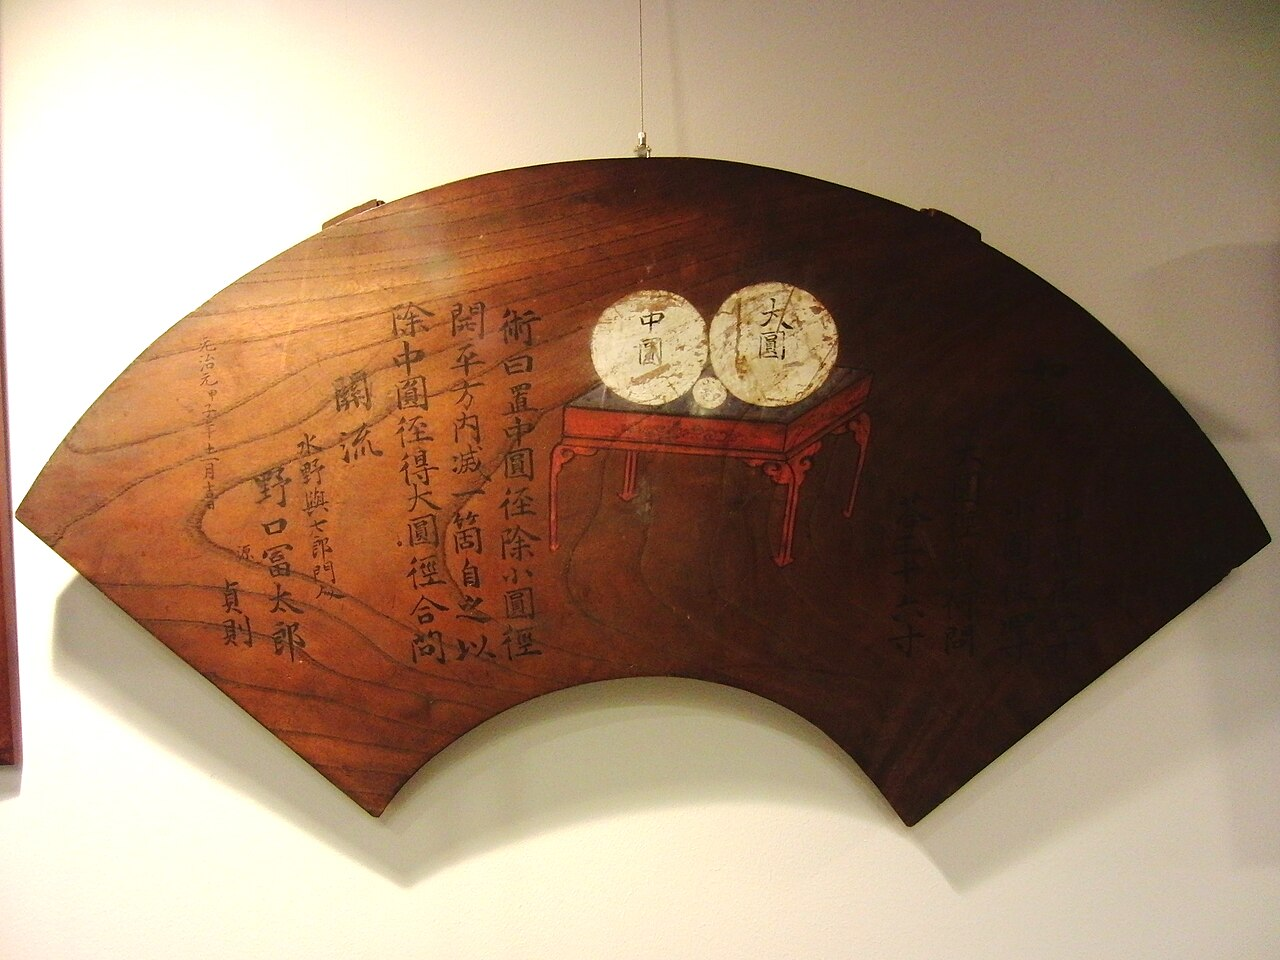
\includegraphics[width=0.78\linewidth,height=0.29\textheight,keepaspectratio]{images/sangaku-konnoh-1864.jpg}
\caption{Tablette sangaku dédiée en 1864 au sanctuaire Konnoh Hachimangu, à Tokyo. Photographie de Momotarou2012, Wikimedia Commons, \href{https://creativecommons.org/licenses/by-sa/3.0/}{CC BY-SA 3.0} ; image reproduite sans modification. Voir la \href{https://commons.wikimedia.org/wiki/File:Sangaku_of_Konnoh_Hachimangu_1864.jpg}{notice de l'image}.}
\end{figure}

Le terme \emph{wasan} désigne la tradition mathématique japonaise. Les méthodes disponibles ne se réduisaient pas à la géométrie à la règle et au compas : calcul numérique, algèbre, tables et techniques de résolution symbolique faisaient partie de l'outillage. Des maîtres itinérants enseignaient le wasan et recopiaient des problèmes rencontrés pendant leurs déplacements.

Pour étudier un sangaku aujourd'hui, on suit une démarche qui respecte l'énoncé et contrôle le dessin :
\begin{enumerate}
 \item identifier exactement les objets, les tangences, les égalités et les points de contact ;
 \item choisir des variables positives et une figure auxiliaire utile ;
 \item transformer la géométrie en relations vérifiables, souvent par Pythagore, similitude ou longueurs de tangentes ;
 \item résoudre l'équation en gardant les contraintes géométriques ;
 \item revenir à la figure afin de vérifier que la solution correspond bien à la configuration voulue.
\end{enumerate}

\section{Problème résolu : trois cercles tangents à une droite}
\textbf{Énoncé.} Deux cercles de rayons $r_1$ et $r_2$ sont tangents extérieurement l'un à l'autre et tangents à une même droite. Un troisième cercle, placé entre eux, est tangent à cette droite et aux deux cercles. Déterminer son rayon $r_3$.

On suppose $r_1,r_2,r_3>0$ et que les points de contact avec la droite sont dans l'ordre correspondant à la figure. La solution dépend uniquement des deux rayons donnés.

\begin{center}
\begin{tikzpicture}[scale=1.35]
  % Figure exacte pour r1 = 2,25 ; r2 = 1 ; r3 = 0,36 (unité : 1 cm sur le dessin)
  % A = (0,0), P = (1.8,0), B = (3,0) : AP = 2*sqrt(r1 r3) = 1,8 ; PB = 2*sqrt(r2 r3) = 1,2 ; AB = 3
  \draw[Forest,very thick] (-2.6,0)--(4.4,0);
  \draw[Ink,thick] (0,2.25) circle (2.25);
  \draw[Ink,thick] (3,1) circle (1);
  \draw[Forest,thick] (1.8,0.36) circle (0.36);
  \coordinate (O1) at (0,2.25); \coordinate (O2) at (3,1); \coordinate (O3) at (1.8,0.36);
  \fill (O1) circle (1.3pt) node[above left] {$O_1$};
  \fill (O2) circle (1.3pt) node[above right] {$O_2$};
  \fill (O3) circle (1pt);
  \draw[dashed] (O1)--(O2); \draw[dashed] (O1)--(O3); \draw[dashed] (O2)--(O3);
  \foreach \p/\n in {0/A,1.8/P,3/B} { \fill (\p,0) circle (1.3pt); \node[below=2pt,font=\small] at (\p,0) {$\n$}; }
  \draw[<->] (-0.35,0.03)--(-0.35,2.22) node[midway,left] {$r_1$};
  \draw[<->] (3.35,0.03)--(3.35,0.97) node[midway,right] {$r_2$};
  \node[font=\small] (lr) at (2.55,-0.45) {$r_3$};
  \draw[->,thin] (lr.north west) -- (2.05,0.18);
\end{tikzpicture}
\end{center}

\subsection{Le lemme de deux cercles}
Soient deux cercles de rayons $a$ et $b$, tangents à une même droite et extérieurement tangents entre eux. Leurs centres sont à des hauteurs $a$ et $b$. Si $d$ est la distance horizontale entre les points de contact à la droite, alors la différence verticale des centres vaut $|a-b|$ et la distance entre centres vaut $a+b$.

Par Pythagore,
\[
 d^2+(a-b)^2=(a+b)^2.
\]
En développant, $(a+b)^2-(a-b)^2=4ab$, donc
\begin{equation}\label{eq:gap}
 d=2\sqrt{ab}.
\end{equation}
Cette formule exprime la distance entre les points où les cercles touchent la droite. Elle reste valable que le centre du premier cercle soit plus haut ou plus bas que le second.

\subsection{Application au petit cercle}
Appliquons (\ref{eq:gap}) d'abord aux deux grands cercles. Si leurs points de contact sont $A$ et $B$, alors
\[
 AB=2\sqrt{r_1r_2}.
\]
Notons $P$ le point de contact du petit cercle avec la droite. Comme le petit cercle est placé entre les deux autres, $AP+PB=AB$. Le même lemme, appliqué à chaque paire grand-petit, donne
\[
 AP=2\sqrt{r_1r_3},\qquad PB=2\sqrt{r_2r_3}.
\]
Par conséquent,
\[
 2\sqrt{r_1r_2}=2\sqrt{r_1r_3}+2\sqrt{r_2r_3}.
\]
Après division par $2$ et mise en facteur de $\sqrt{r_3}$ :
\[
 \sqrt{r_1r_2}=\sqrt{r_3}(\sqrt{r_1}+\sqrt{r_2}).
\]
Les rayons étant positifs, on peut élever au carré et obtenir
\begin{equation}\label{eq:radius}
 \boxed{r_3=\frac{r_1r_2}{(\sqrt{r_1}+\sqrt{r_2})^2}}.
\end{equation}

\begin{exemple}[Calcul numérique]
Prenons $r_1=36$ et $r_2=9$, en centimètres. Alors $\sqrt{r_1}=6$, $\sqrt{r_2}=3$, et
\[
 r_3=\frac{36\cdot9}{(6+3)^2}=\frac{324}{81}=4\text{ cm}.
\]
Vérification géométrique : $AB=2\sqrt{36\cdot9}=36$ cm ; les deux morceaux valent $AP=2\sqrt{36\cdot4}=24$ cm et $PB=2\sqrt{9\cdot4}=12$ cm. La somme $24+12=36$ confirme la position du petit cercle.
\end{exemple}

\section{Une variable qui rend la formule plus simple}
La formule (\ref{eq:radius}) peut paraître surprenante. Posons $q_i=1/\sqrt{r_i}$. En prenant la racine carrée puis l'inverse dans (\ref{eq:radius}), on trouve
\begin{equation}\label{eq:q}
 \boxed{q_3=q_1+q_2},\qquad\text{c'est-à-dire}\qquad
 \frac{1}{\sqrt{r_3}}=\frac{1}{\sqrt{r_1}}+\frac{1}{\sqrt{r_2}}.
\end{equation}
La géométrie non linéaire des rayons devient une addition simple dans la variable $q$. Si $r_1=r_2=r$, alors
\[
 \frac{1}{\sqrt{r_3}}=\frac{2}{\sqrt r},\qquad r_3=\frac r4.
\]
Deux cercles égaux se touchant l'un l'autre sur une droite laissent donc entre eux une place pour un cercle de rayon égal au quart du leur.

\subsection{Insertion répétée}
On peut réutiliser la même construction dans les espaces curvilignes qui restent. Si deux cercles de rayons égaux à $r$ ont laissé un cercle de rayon $r/4$, alors, pour une nouvelle insertion entre un cercle de rayon $r$ et celui de rayon $r/4$, l'équation en $q$ donne
\[
 q_{\mathrm{nouveau}}=\frac1{\sqrt r}+\frac1{\sqrt{r/4}}=\frac3{\sqrt r},
 \qquad r_{\mathrm{nouveau}}=\frac r9.
\]
Cette suite n'est pas une approximation graphique : elle résulte de la même relation exacte à chaque étape.

\subsection{Limites et prudence}
La formule suppose que les trois cercles sont du même côté de la droite, que les deux cercles extérieurs sont tangents entre eux, et que le troisième se trouve entre leurs points de contact. Si les cercles se chevauchent, si le cercle recherché est placé à l'extérieur ou si une tangence est intérieure, l'addition $AP+PB=AB$ peut ne plus décrire la figure. Il faut alors repartir de l'énoncé et ajuster les équations de distance.

\section{Pourquoi ces problèmes sont-ils instructifs ?}
Les configurations de tangence transforment une image riche en quelques contraintes précises. Une tangence entre deux cercles donne une distance entre centres ; une tangence à une droite donne une hauteur égale au rayon ; une tangence double fournit souvent un triangle rectangle. Le dessin suggère alors Pythagore.

Ce problème illustre une méthode générale de modélisation géométrique :
\begin{enumerate}
 \item nommer les centres et les rayons ;
 \item projeter les centres sur la droite de contact ;
 \item écrire le triangle rectangle des centres ;
 \item simplifier l'identité obtenue avant de remplacer les nombres ;
 \item vérifier la solution sur les distances de la figure.
\end{enumerate}

Un dessin n'est jamais une preuve de tangence. Deux cercles peuvent sembler toucher à l'écran sans que leurs centres soient à la somme de leurs rayons. Les égalités de distance sont la partie mathématique essentielle.

\subsection{Exercices et réponses}
\begin{enumerate}
 \item Si $r_1=16$ et $r_2=4$, trouvez $r_3$.
 \item Pour quelles valeurs de $r_1,r_2>0$ le petit cercle a-t-il un rayon $r_3=1$ ?
 \item Expliquez pourquoi la valeur de $r_3$ est toujours strictement plus petite que chacun des rayons $r_1,r_2$.
 \item Démontrez (\ref{eq:gap}) en plaçant les centres en $(0,a)$ et $(d,b)$.
\end{enumerate}
\textbf{Réponses.}
\begin{enumerate}
 \item $r_3=\dfrac{16\cdot4}{(4+2)^2}=\dfrac{64}{36}=\dfrac{16}{9}$. Vérification avec (\ref{eq:q}) : $\frac14+\frac12=\frac34=\frac1{\sqrt{r_3}}$, donc $r_3=\frac{16}{9}$. (La valeur $r_3=1$ correspond à $r_1=r_2=4$.)
 \item Il faut $\dfrac1{\sqrt{r_1}}+\dfrac1{\sqrt{r_2}}=1$. Cela impose $r_1>1$ et $r_2>1$, et donne $r_2=\bigl(\sqrt{r_1}/(\sqrt{r_1}-1)\bigr)^2$. Par exemple $r_1=r_2=4$, ou $r_1=9$ et $r_2=9/4$.
 \item Par (\ref{eq:q}), $1/\sqrt{r_3}=1/\sqrt{r_1}+1/\sqrt{r_2}>1/\sqrt{r_1}$, donc $r_3<r_1$ ; de même $r_3<r_2$.
 \item Avec $O_1=(0,a)$ et $O_2=(d,b)$, la tangence extérieure donne $d^2+(a-b)^2=(a+b)^2$, donc $d^2=4ab$ et $d=2\sqrt{ab}$.
\end{enumerate}

\section*{Références}
\begin{enumerate}
 \sourceweb{National Diet Library of Japan, \og Sangaku (Mathematical Tablet)\fg{}, histoire, tablettes et exemple géométrique}{https://www.ndl.go.jp/math/e/s1/c5.html}
 \sourceweb{T. Rothman, \og Sangaku Problems About Ellipses: Why Primary Sources Matter\fg{}, The Mathematical Intelligencer}{https://link.springer.com/article/10.1007/s00283-021-10105-6}
 \sourceweb{Mansur, \og Japanese Sangaku: Geometry Displayed in Temples\fg{}, problème pédagogique de trois cercles tangents}{https://history-math.org/publications/hm-tt-5c1d88688388-en/}
\end{enumerate}
\end{document}
